\documentclass[
	%a4paper, % Use A4 paper size
	letterpaper, % Use US letter paper size
]{jdf}

\addbibresource{references.bib}

\author{Nan Xiao}
\email{nanx@gatech.edu}
\title{CS6750 HCI Summer 2021:\\Assignment P1}

\begin{document}
%\lsstyle

\maketitle

\begin{abstract}
	In this assignment P1, views of the user (processor, predictor) are compared for a Canvas task. Then participant view of the user is studied for a video conferencing app - Zoom. Next, feedback cycles (gulf of execution, gulf of evaluation) are discussed for the Canvas task - submitting an assignment. Finally, a regular life inconvenience caused by gulf of execution or gulf of evaluation is studied and compared with a similar activity but different task.
\end{abstract}

\section{Views of the user: Processor vs Predictor model}
In this section, we compare the views of the user for the Canvas task - checking grades. Both processor model and predictor model are studied and compared. Grades are important for OMSCS students since most of the classes are non-curve based and student are expected to have at least B (80/100) in average for all classes. So it is important for a student to understand how good he/she performs through out the whole course. However, it is not always an easy task for a student to track how good he performs so far.

\begin{figure}[h]
	\centering
	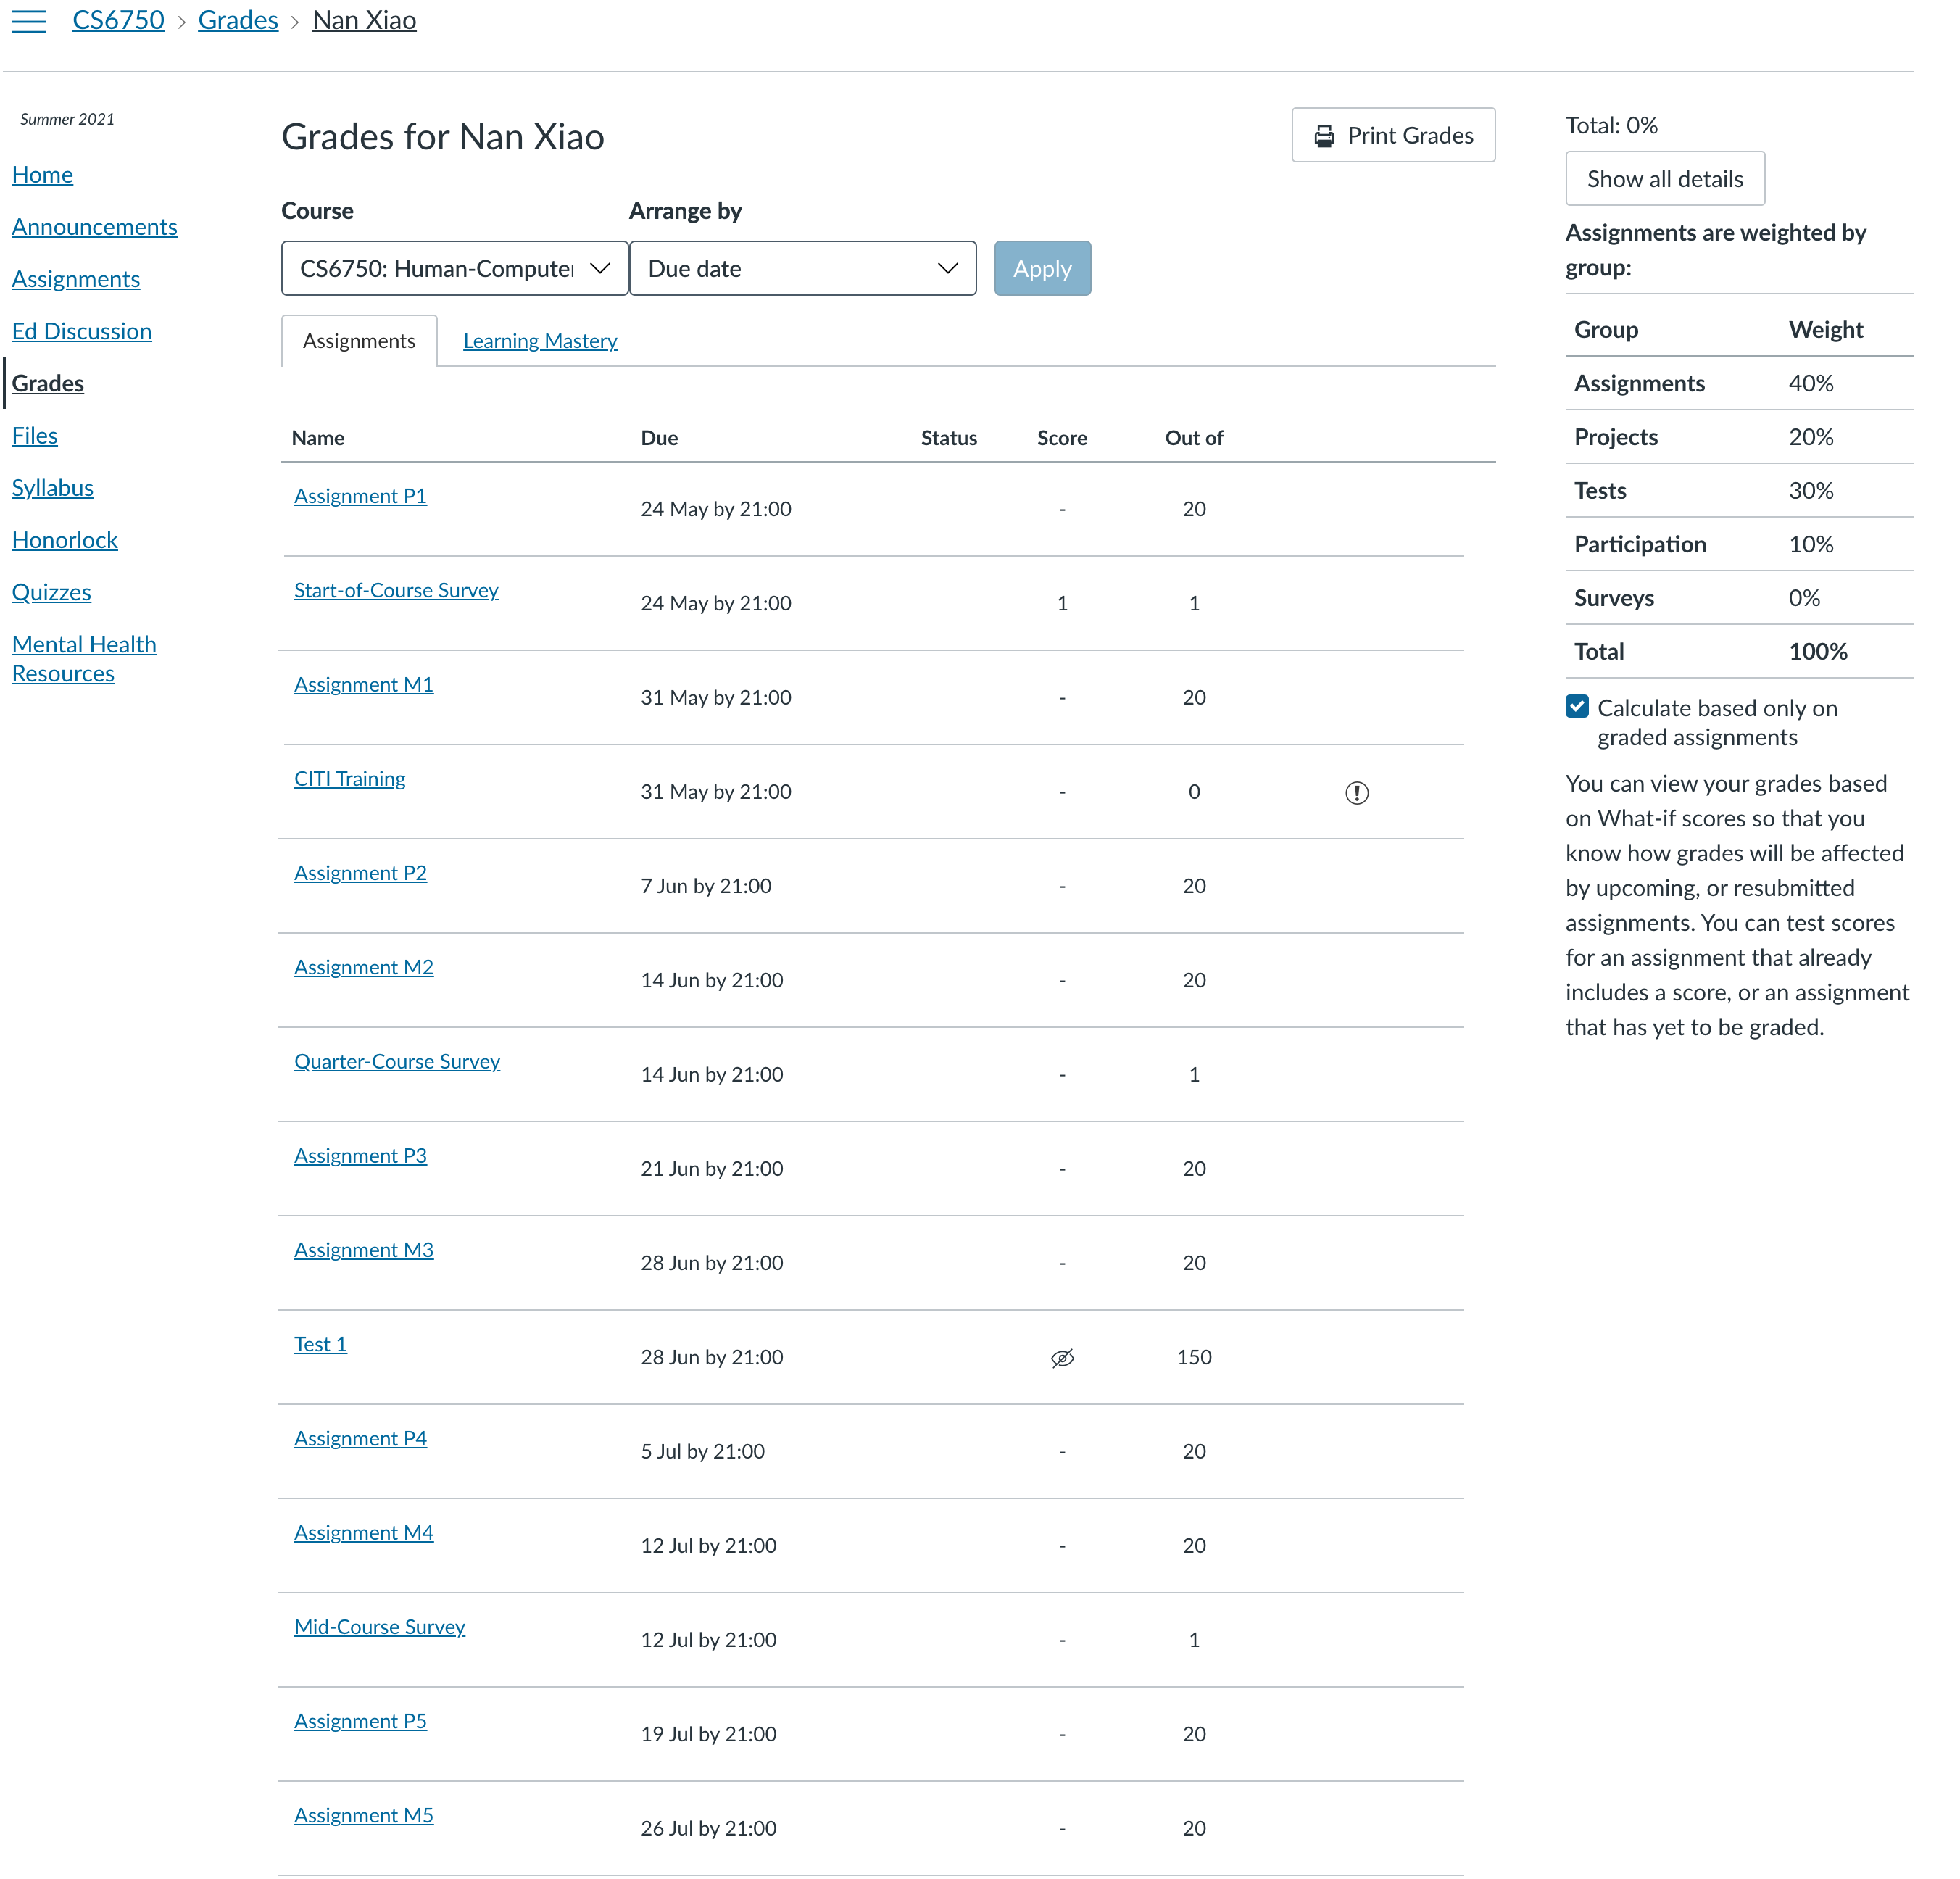
\includegraphics[height=6cm]{Figures/canvas_grades.png}
	\caption{The Grades interface of Canvas app}
	\label{fig:canvas_grades}
\end{figure}

\subsection{Processor model}
In the processor model, we assume the interface should be designed that it fits in whatever a user knows to do. The user lands on the grades page is assumed to have expert knowledge of the interface and thus he/she will perform the task as expected. The objective is to find out whether the student is going to get a A, B or C in the course based on grades. It can be measurable in such way that if the percentage score in the canvas matches final grade (A -> 90\% and above, B -> 80\% and above and etc.), the task is considered as done. Otherwise, it is considered as failed (as shown in figure 2, the final grade is A while in grades page it only has 67.62\% score). In this model, we can use the historical data to test whether the percentage score of canvas page matches the final score, and the result is unbiased. It is a great way to quantitatively evaluate the existing interface performance and do optimization accordingly. But processor model fails to take the user into consideration in the design, a junior and a senior student may have different probability to complete the task. Also, it does not understand why a task succeeds or fails. So it cannot find the reason or cause of failure to redesign the interface.

\begin{figure}[h]
	\centering
	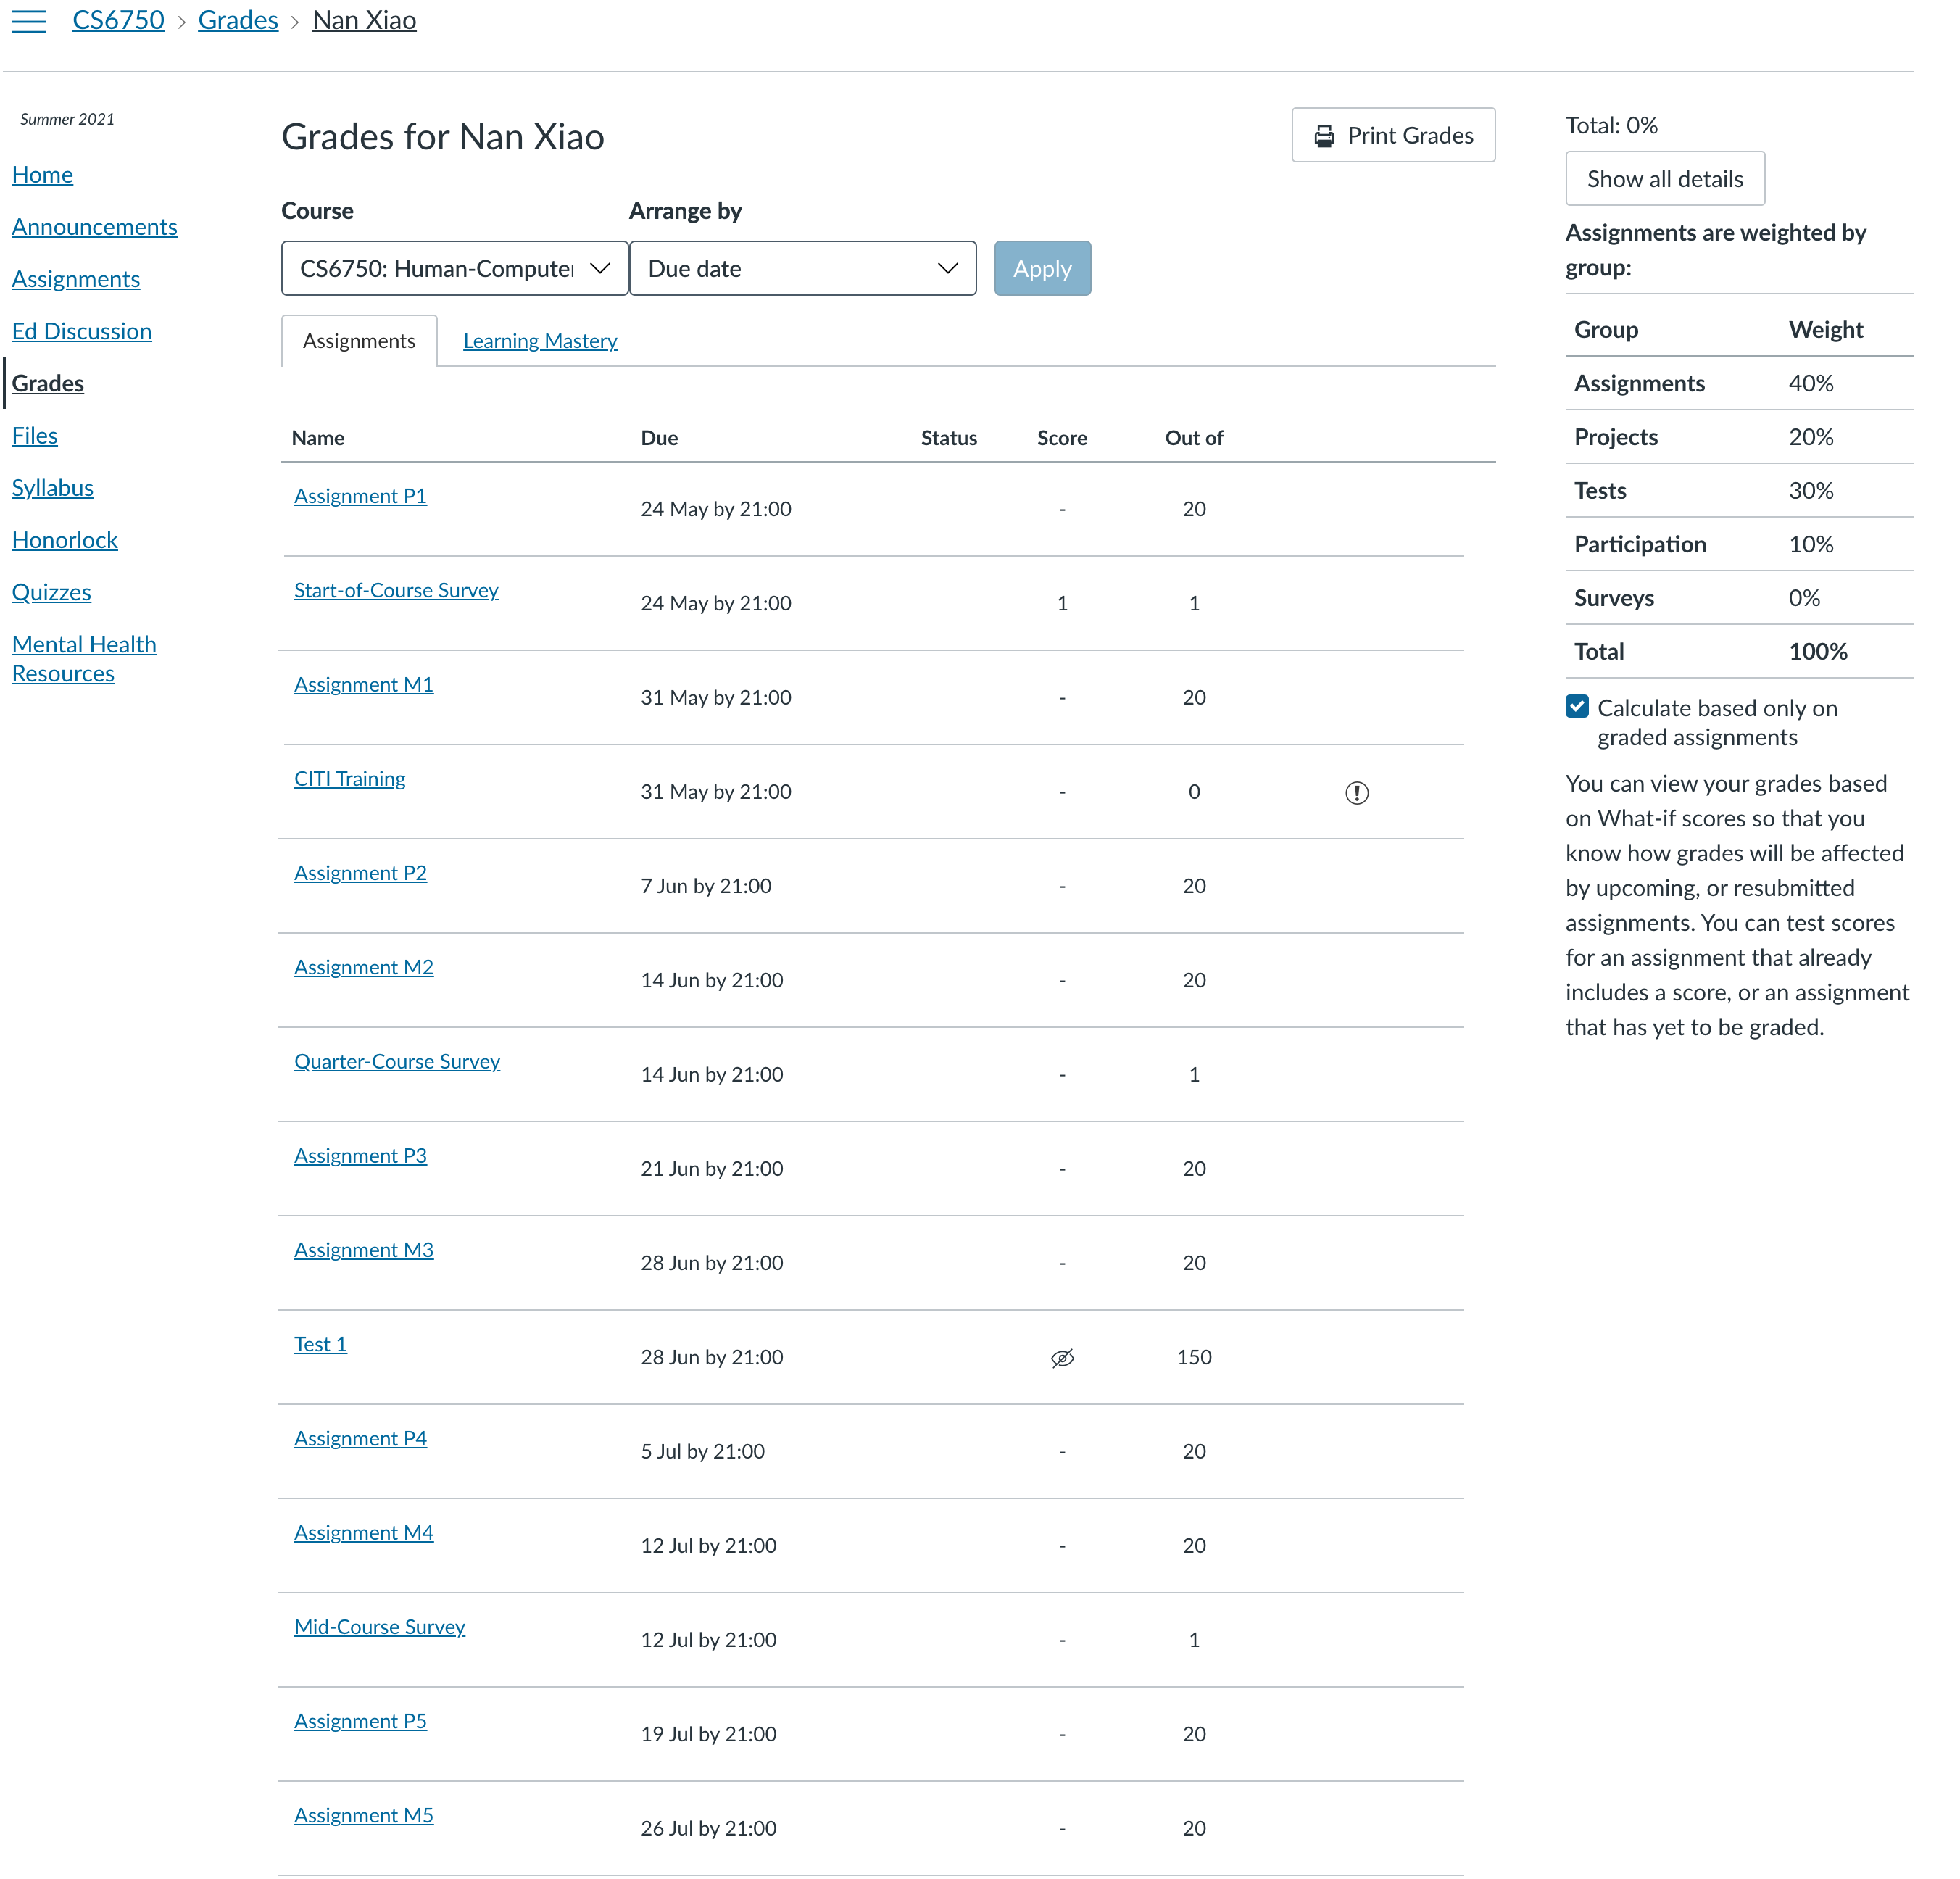
\includegraphics[height=6cm]{Figures/canvas_grades.png}
	\caption{The grades has no relation to the final score}
	\label{fig:canvas_grades}
\end{figure}

\subsection{Predictor model}
In the predictor model, we take the user into consideration. A junior student may need more help in understanding how to use the interface while a senior student may already know how to get the task done. So there should be a on-boarding guide in the grade interface for the novice user. Also, the users are more concerned with grades related assignments instead of all items, so there should be a filter for the user to see only items related to the grades. Finally, there are chances one lowest score of a category is dropped, so user would expect to adjust that in the interface instead of using all scores. The user would expect the final weighted score as close as possible to the real score and that he/she can calculate how much the rest of assignments score needed. Since the user needs to link the percentage score on Canvas to the final course score, the interface should be capable to make the suggestion as well. Especially when the course is still on-going, the interface should be able to suggest an assignment score for up-coming assignments as well to make the user have a better estimation of the final score. Because of the qualitative design, it is much harder to analyze whether the interface is better or worse, and it is prone to biases. Also, predictor model would fail in the cases when context matter to the task. As the example shown in the class, the Tesla navigation app needs to take environment into consideration.[1] In this case, the online students and in-class students would have different contexts and in-class students are more likely to find help to understand how to use the interface. Thus even the novices can have the experts help.

\subsection{Comparison}
In the below table we can see the comparison of processor model vs predictor model according to the lecture by David Joyner.[1] 

\begin{table}[h] % [h] forces the table to be output where it is defined in the code (it suppresses floating)
	\caption{Comparison Between Processor model and Predictor model}
	\small % Reduce font size
	\centering % Centre the table
    \begin{tabular}{|l|l|l|}
    \hline
    \textbf{Name} & \textbf{Processor model}                                                                       & \textbf{Predictor model}                                                                         \\ \hline
    Requirement   & Fit within human limits                                                                        & Fit within user's knowledge                                                                      \\ \hline
    Evaluation    & Quantitative experiments                                                                       & Qualitative studies                                                                              \\ \hline
    Pros          & \begin{tabular}[c]{@{}l@{}}Objective comparisons \\ May use existing data\end{tabular}         & \begin{tabular}[c]{@{}l@{}}Fuller picture \\ May target novices\end{tabular}                     \\ \hline
    Cons          & \begin{tabular}[c]{@{}l@{}}Expert-focused\\ What not Why\\ Optimize, not redesign\end{tabular} & \begin{tabular}[c]{@{}l@{}}Expensive to analyze\\ Prone to biases\\ Ignores context\end{tabular} \\ \hline
    \end{tabular}
\end{table}

From the insights of previous 2 sections we can see that processor model and predictor model would give different suggestion to improve the interface. Using processor model, we will optimize the existing interface, for example showing the total score in the first page top section, or always using a coefficient 0.8 ~ 1.2 times the Canvas score according to the difficulty of the course. But using predictor model, we will optimize the interface based on users' expert levels. We can have a guide for the novices while more customization for expert to adjust weights of the scores. But often it is better to gain insights using predictor model and measure using processor model. The 2 models perform best when work together.

\section{View of the user: Participant model}
Since COVID-19, there are lock-downs in the cities. We mainly shift work and even social to video conference platform. Zoom is one of the most popular choices. In this section, we will take the participant view of the user to study the Zoom interface in multiple contexts. The participant model will take not only the user but also the context into consideration.

\begin{figure}[h]
	\centering
	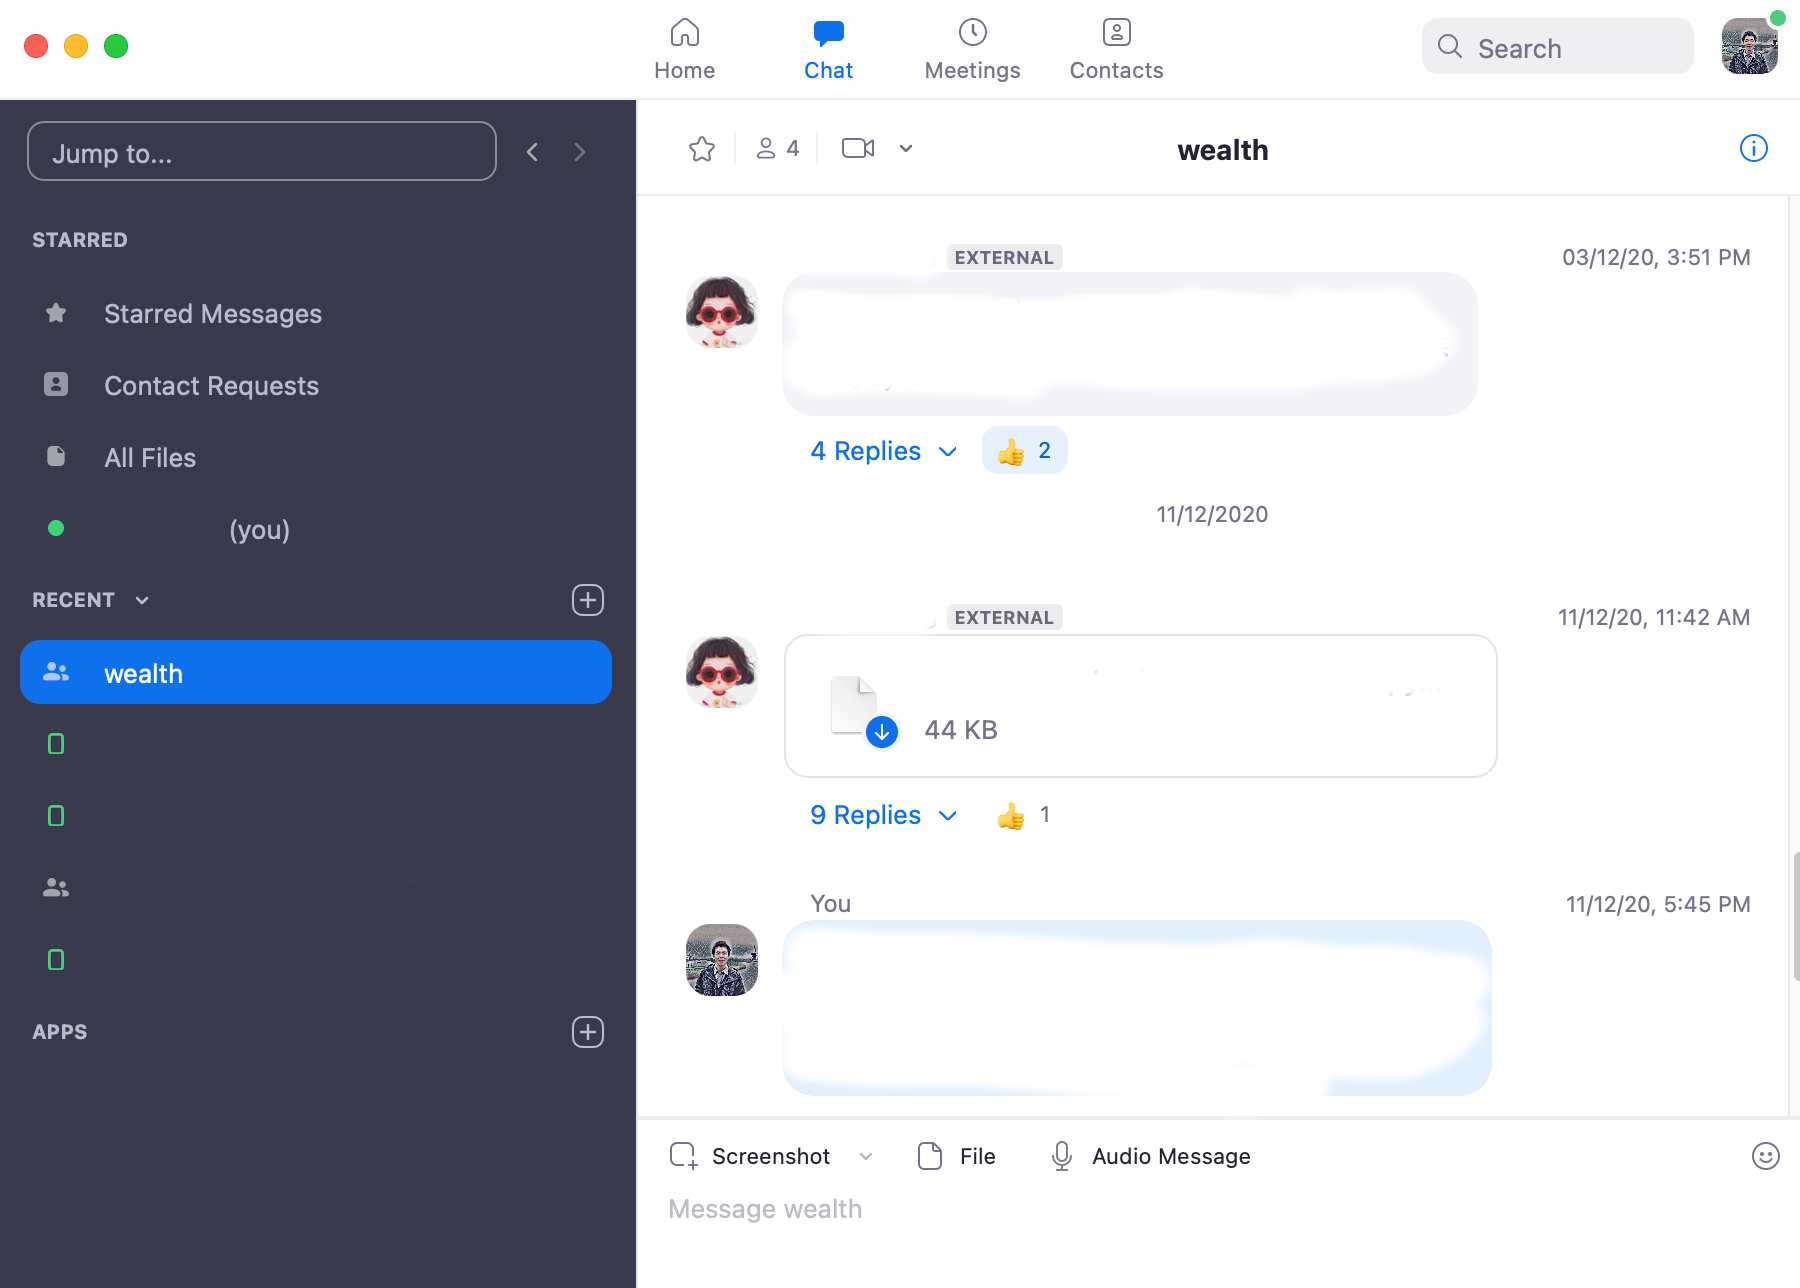
\includegraphics[height=6cm]{Figures/zoom.jpg}
	\caption{Zoom Interface in Mac}
	\label{fig:zoom}
\end{figure}

\subsection{Task with multiple contexts}
People use the video conference app in different contexts, and in different devices as well. We are focusing on the video conference task here. First, people are all work from home while having the video conference. Second, people can be driving or in public transportation while having the video conference. Third, people can have video conference with friends instead of colleagues. Last, people can have video conference directly with one person instead of a group of people. There are all common contexts for video conferences while they should be handled differently by the interface.

\subsection{How contexts affect task}
These contexts pose different challenges to the video conferencing tasks. First, when people all work from home, the background may not be appropriate for a business meeting. Second, when people are in transportation, their videos may be unstable and shaky, which is challenging for the other side to watch and focus on the content (task). Third, people having video calls with friends are more relaxed seldom need to share screen for a presentation. Last, the interface should design in a different way when showing one person versus showing 50 people.

\subsection{Context adapted interface}
The interface should be designed differently for different context. First, when people are working from home instead having meetings in the office, there should be a professional virtual background. Second, when people are having meeting using the mobile device, the interface should have a build-in stabilizer. Third, when people using the interface with friends, it should remove all the business functions but add functions like filters or AR that can be used casually. Last, the interface should adapt to the number of users that each window of user gets smaller when number of participants gets larger.

\begin{figure}[h]
	\centering
	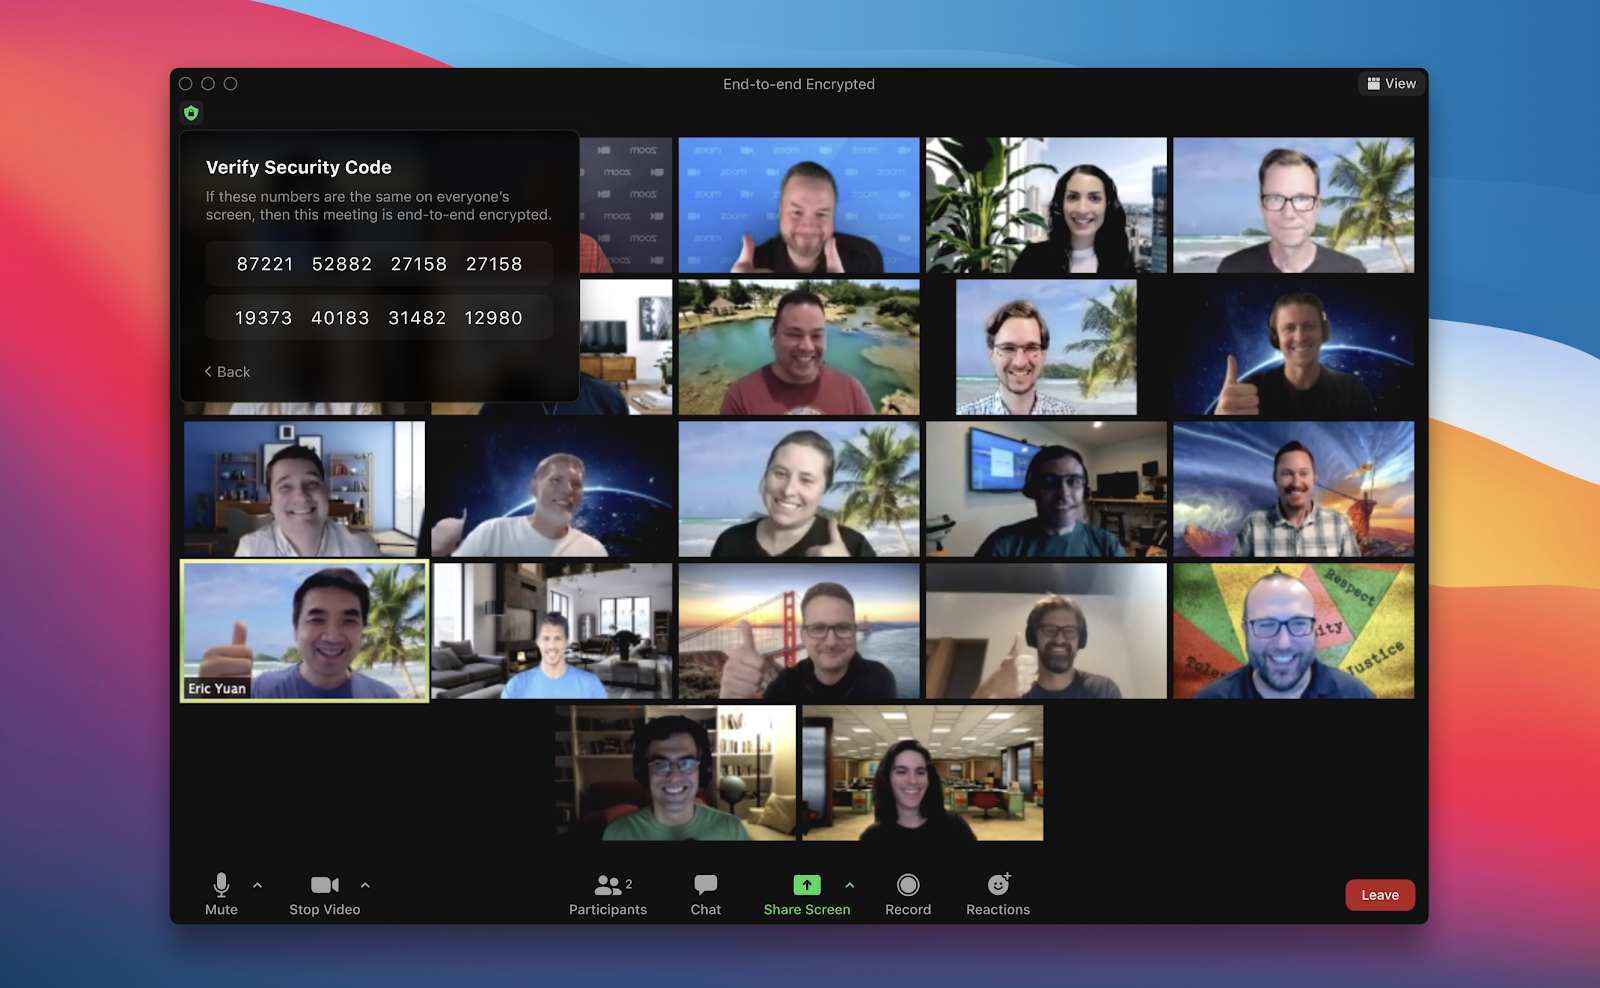
\includegraphics[height=6cm]{Figures/Zoom-End-to-End.png}
	\caption{Zoom group meeting interface Source: \href{https://blog.zoom.us/zoom-rolling-out-end-to-end-encryption-offering/}{Zoom-blog}.}
	\label{fig:zoom_group}
\end{figure}

\begin{figure}[h]
	\centering
	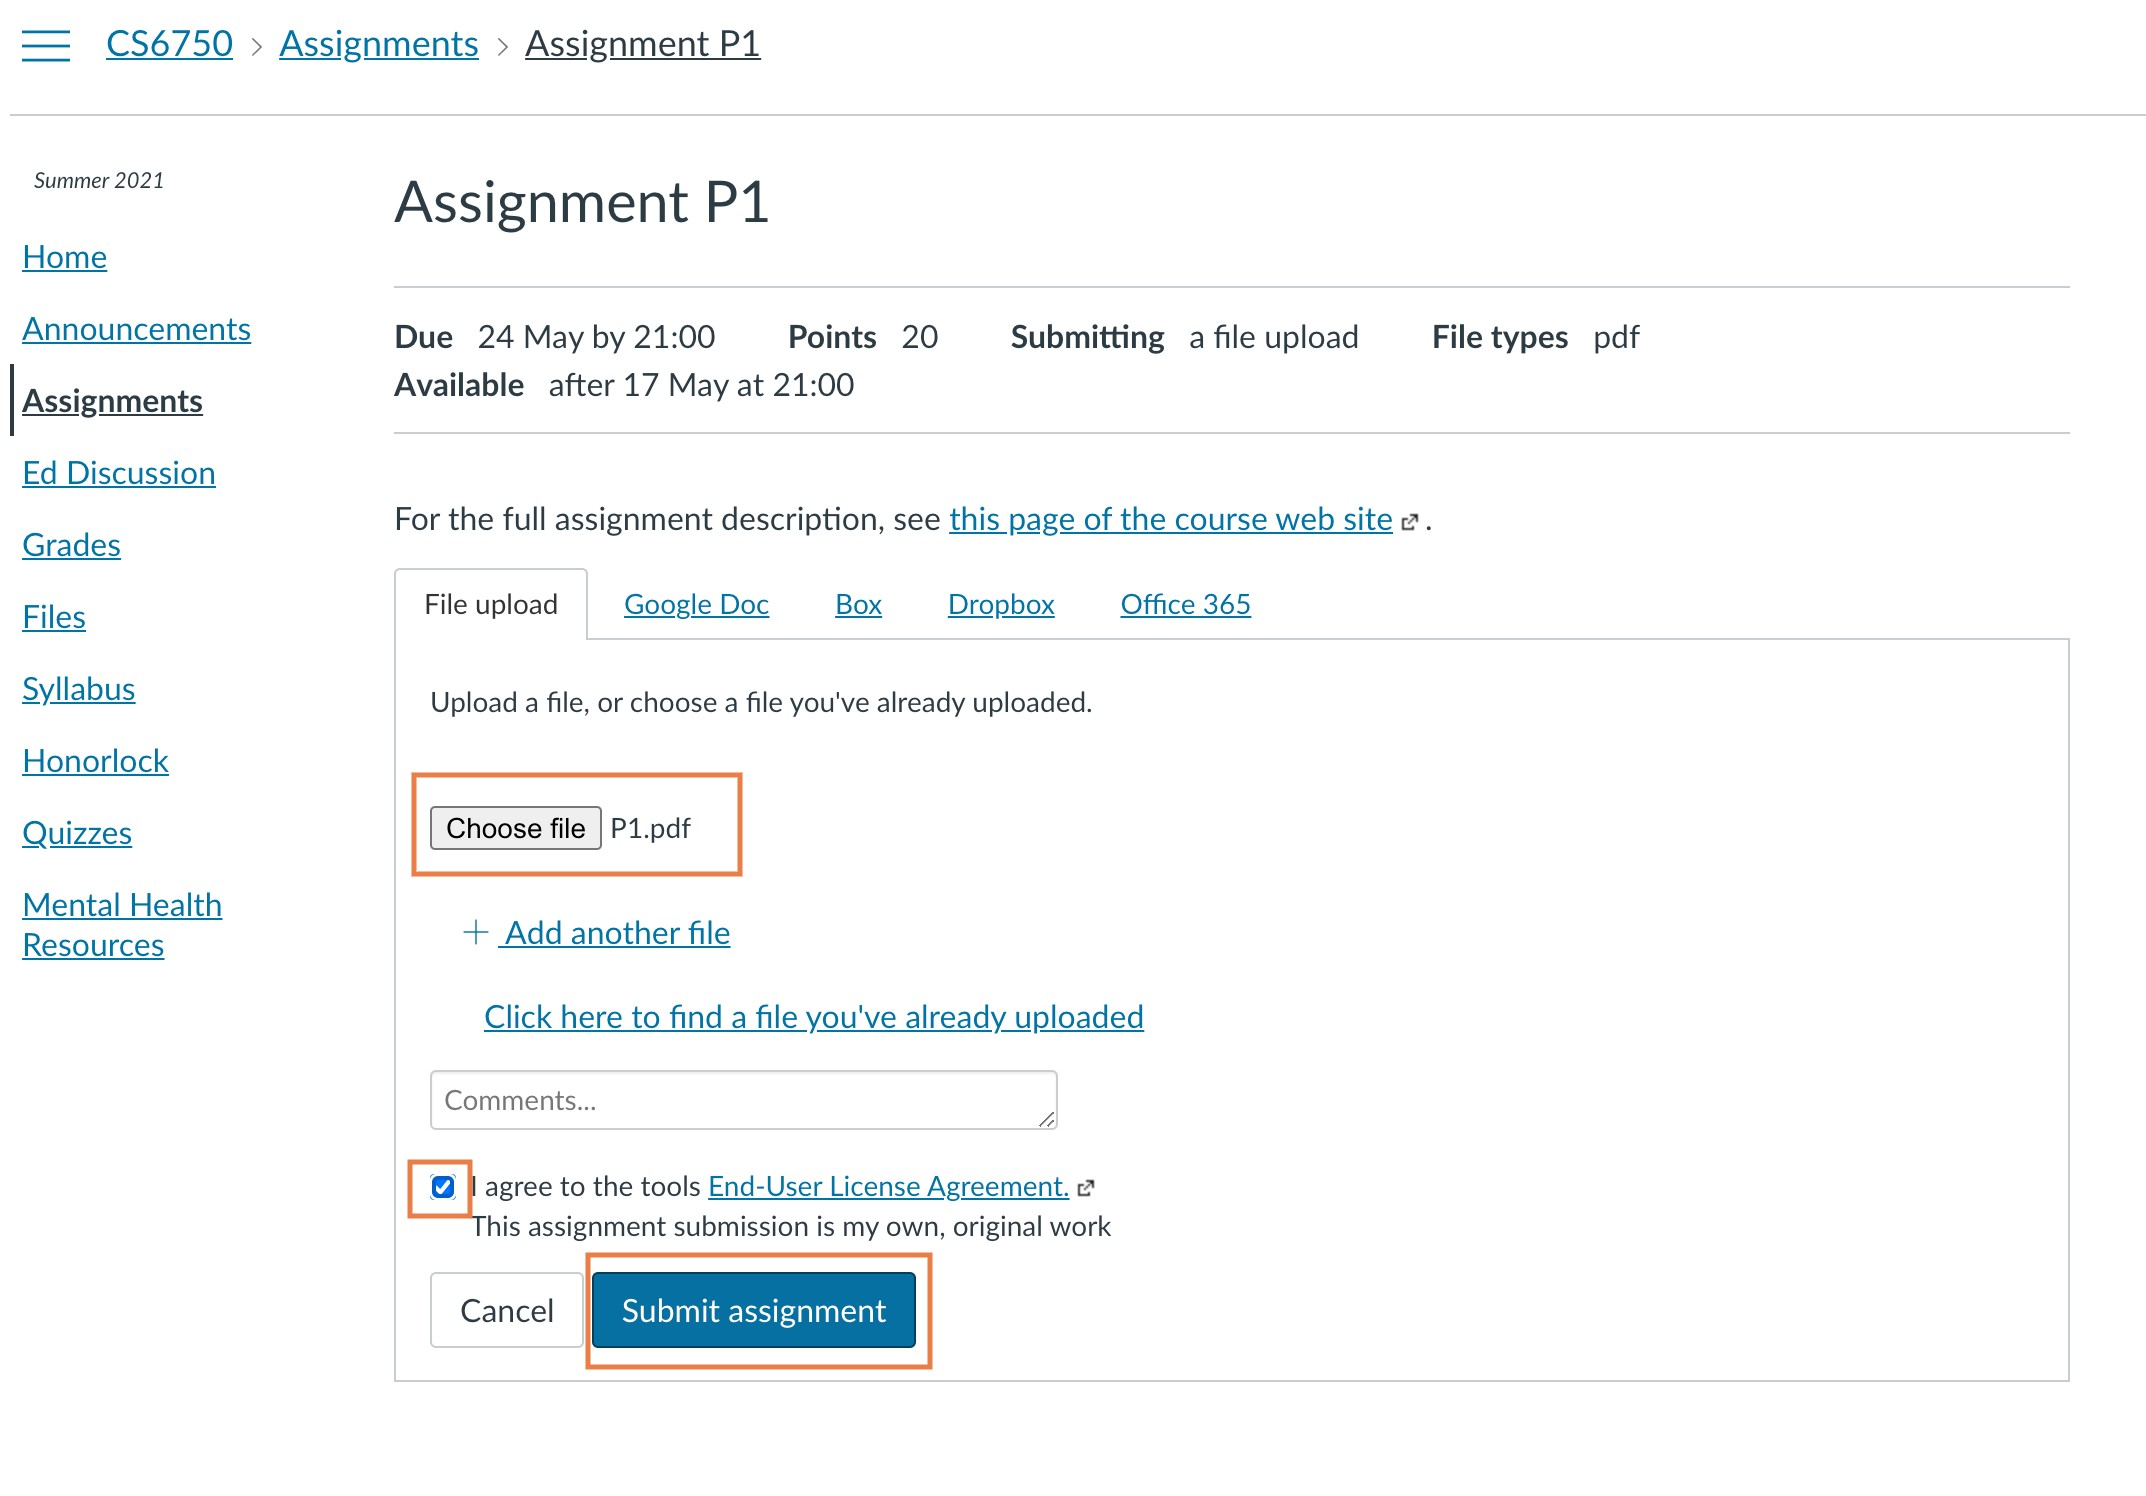
\includegraphics[height=6cm]{Figures/upload_assignment.jpg}
	\caption{Multiple steps before submission}
	\label{fig:upload_assignment}
\end{figure}

\section{Canvas Submission task}
Canvas submission task is studied here to evaluate the gulf of execution and gulf of evaluation. Generally, it is hard to submit the assignment but easy to evaluate whether the task is successful or not.

\subsection{Gulf of execution}
In the Canvas submission task, the user needs to take many steps to reach to the submission page. Also, he/she needs to understand all steps correctly before he/she can successfully submit his/her assignment. It is easy to identify the intention, but hard to identify the actions or how to execute in the interface. Figure 5 shows the gulf of execution for submission. If the user has no prior knowledge, there is a chance that he/she may not be able to submit this task.

\subsection{Gulf of evaluation}
Canvas submission has a good interface to tell user the submission is successful using the status update in the figure shown below. It also shows a timestamp for the user to understand when the task is done. This is crucial since the user may update the work and would like to submit the latest version. This timestamp helps the user to understand which version he/she is submitted to the Canvas. Also, the interface indicates the name of assignments, and allow user to download the submitted work to verify. This further allows the user to evaluate whether the work he/she submitted is as expected. It is easy to evaluate and interpret from the interface output.

\begin{figure}[h]
	\centering
	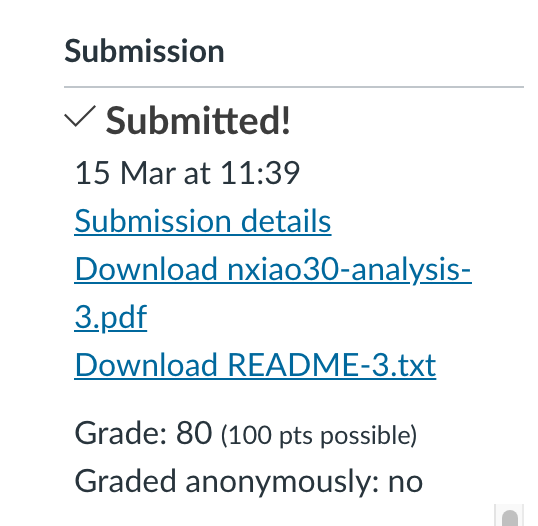
\includegraphics[height=6cm]{Figures/canvas_submit_eval.png}
	\caption{Status update for submitted assignment}
	\label{fig:canvas_submit_eval}
\end{figure}

\section{Gulf caused by weak interface}
In this section, we will discuss about the gulf caused by poorly designed interface of a investment website FSM. Then compare with a better designed interface of Grab.

\subsection{Failure of the current interface}
The FSM website is used for fund investment. Users can buy and sell funds on the platform. One poor interface for FSM is that it is difficult to find out how to deposit to the platform. One needs to navigate through dozens of options before he/she can arrive the final instruction page about how to transfer funds. Even in the final page, one needs to scroll down multiple pages to find the useful information. And it is not able to transfer fund using the app, but instead, you have to log on to the personal internet banking to do the fund transfer. It introduces a large gulf of execution. Furthermore, when one finish transfer through internet banking, it took hours to confirm the transaction. That introduces a gulf of evaluation. The user may have no idea for a while whether the task is successful or not.

\begin{figure}[h]
	\centering
	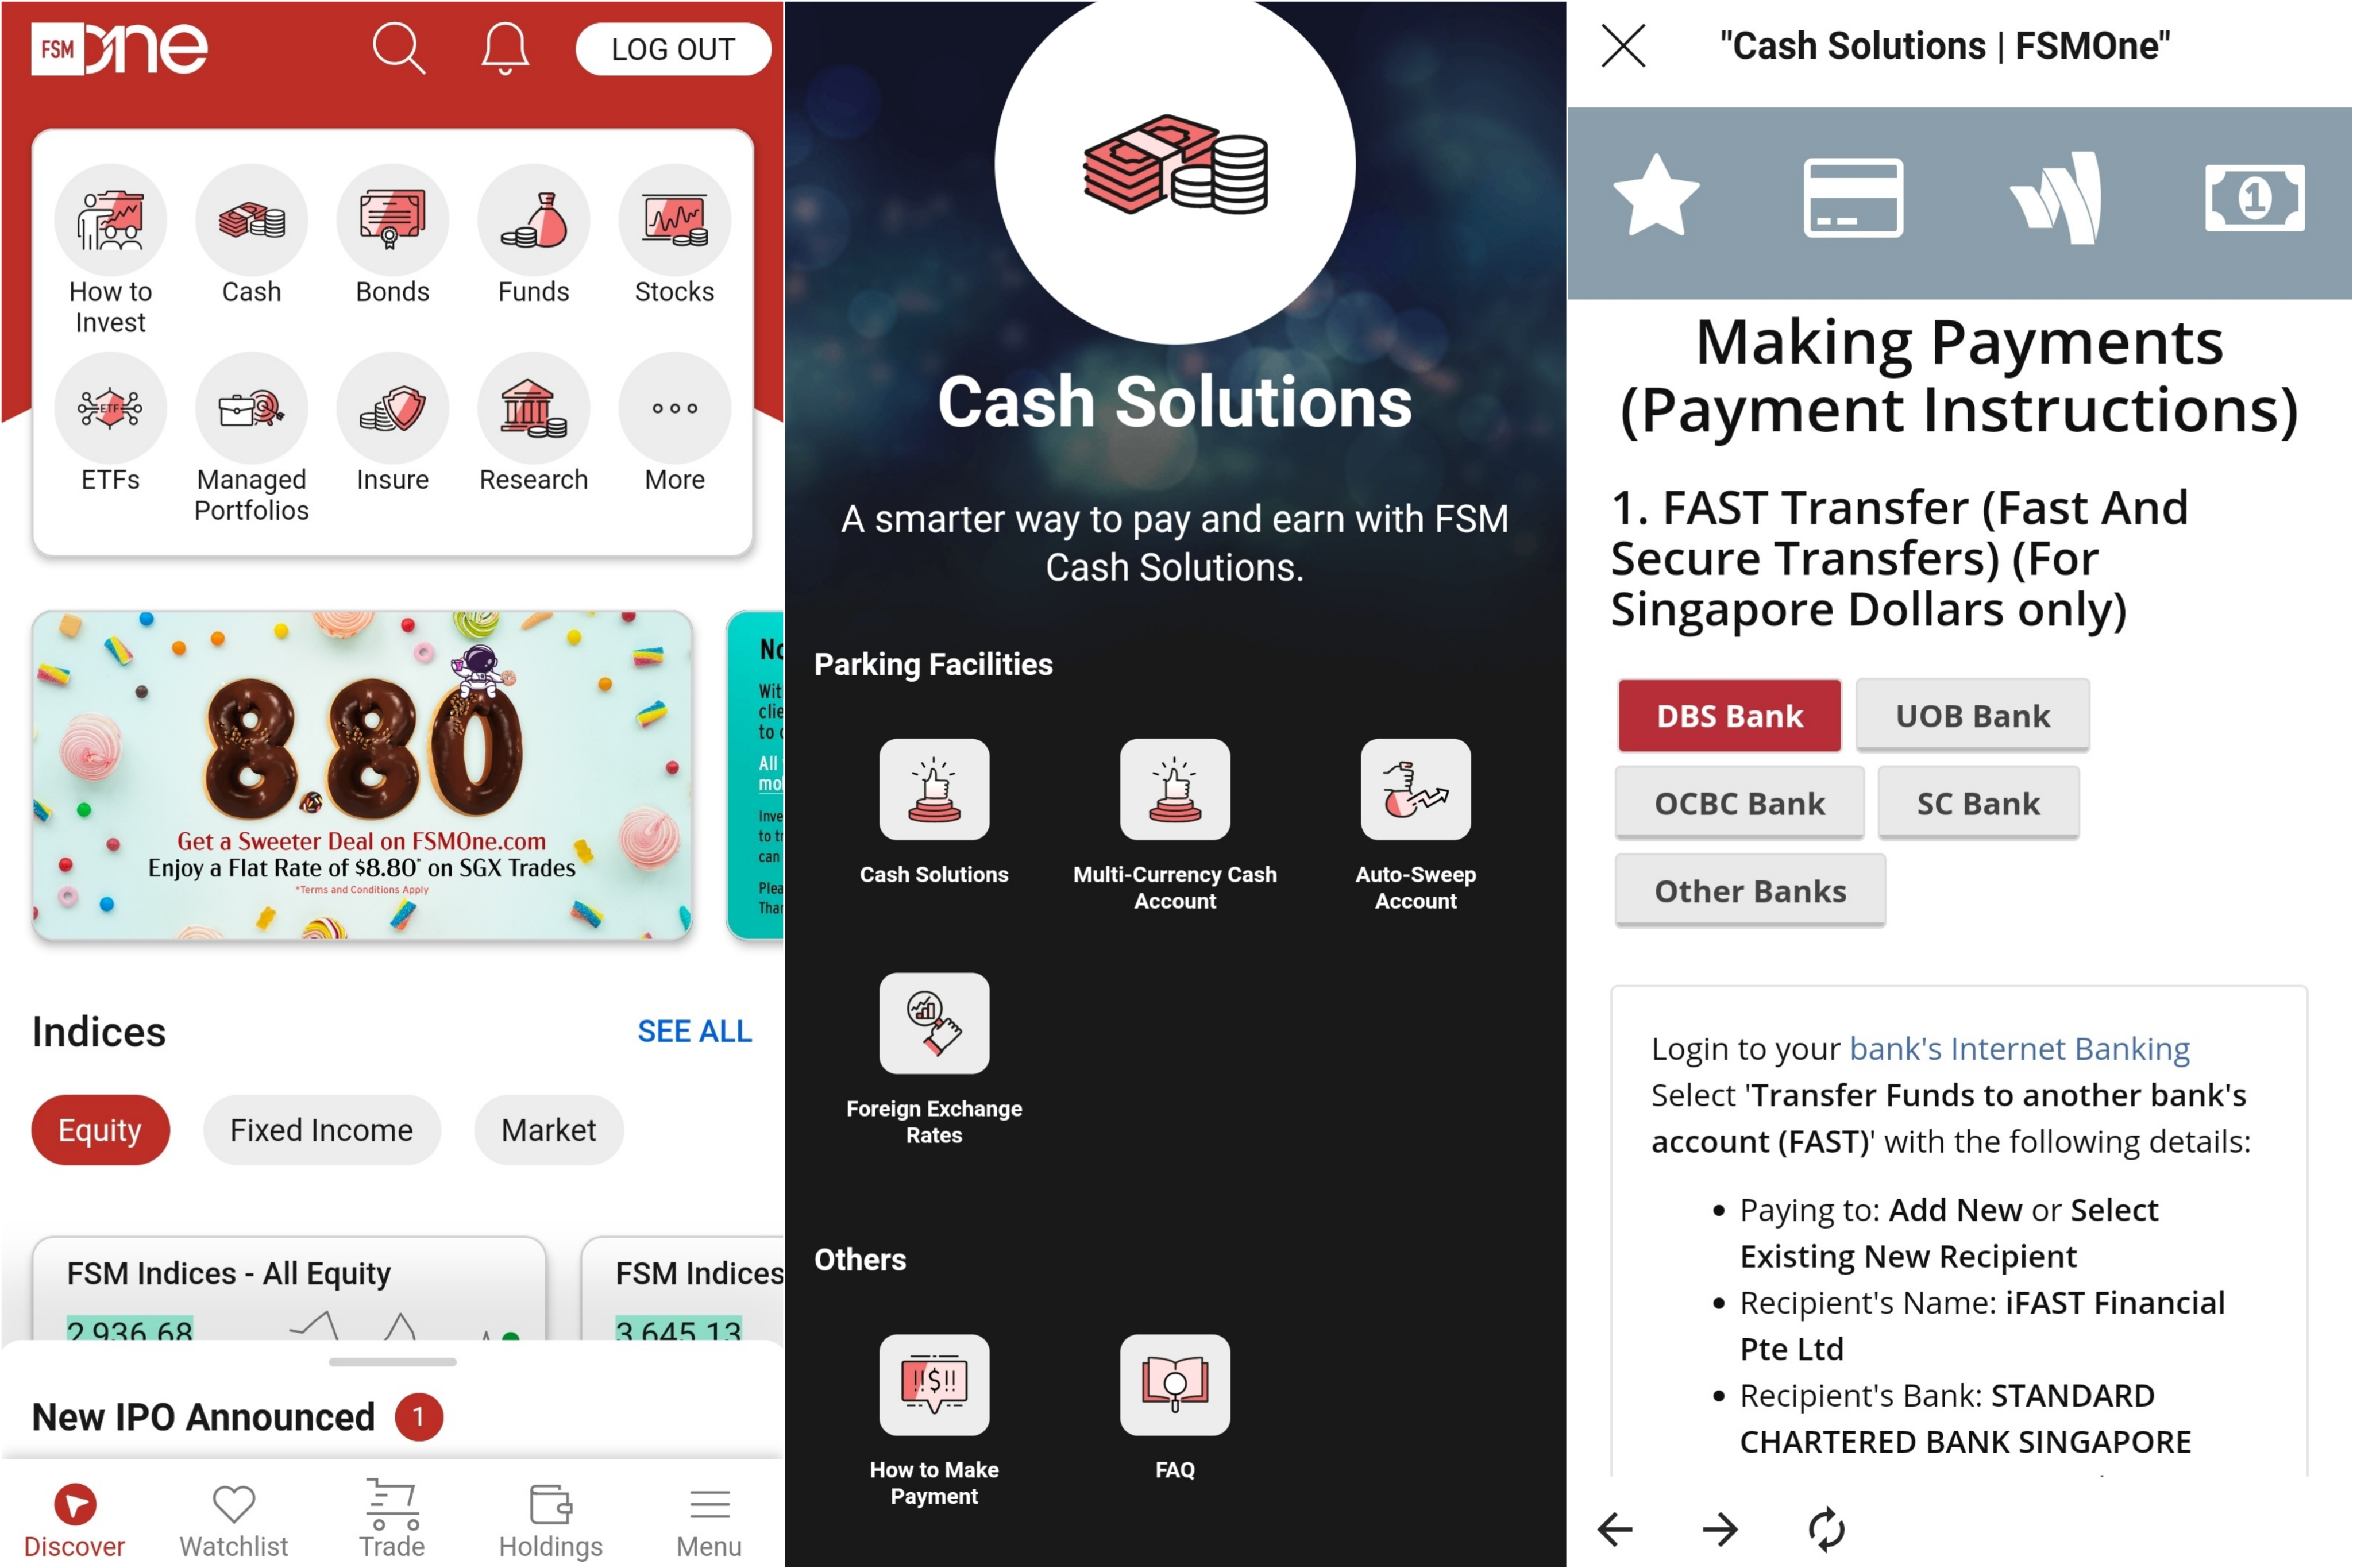
\includegraphics[height=6cm]{Figures/fsm_one.jpg}
	\caption{The flow to find top-up option in FSM ONE app}
	\label{fig:fsm_one}
\end{figure}

\subsection{Similar task with better interface}
For the similar task of transferring funds in Grab, the interface does a much better job. One can easily find the wallet in the top left corner, and the "Top-up" option is very obvious for the user to select. The transfer is done in the app, with immediate feedback that the transaction is successful. The user can verify that wallet balance is updated accordingly as well. Both execution and evaluation happen as the user expected. This eliminates both gulf of execution and gulf or evaluation.

\begin{figure}[h]
	\centering
	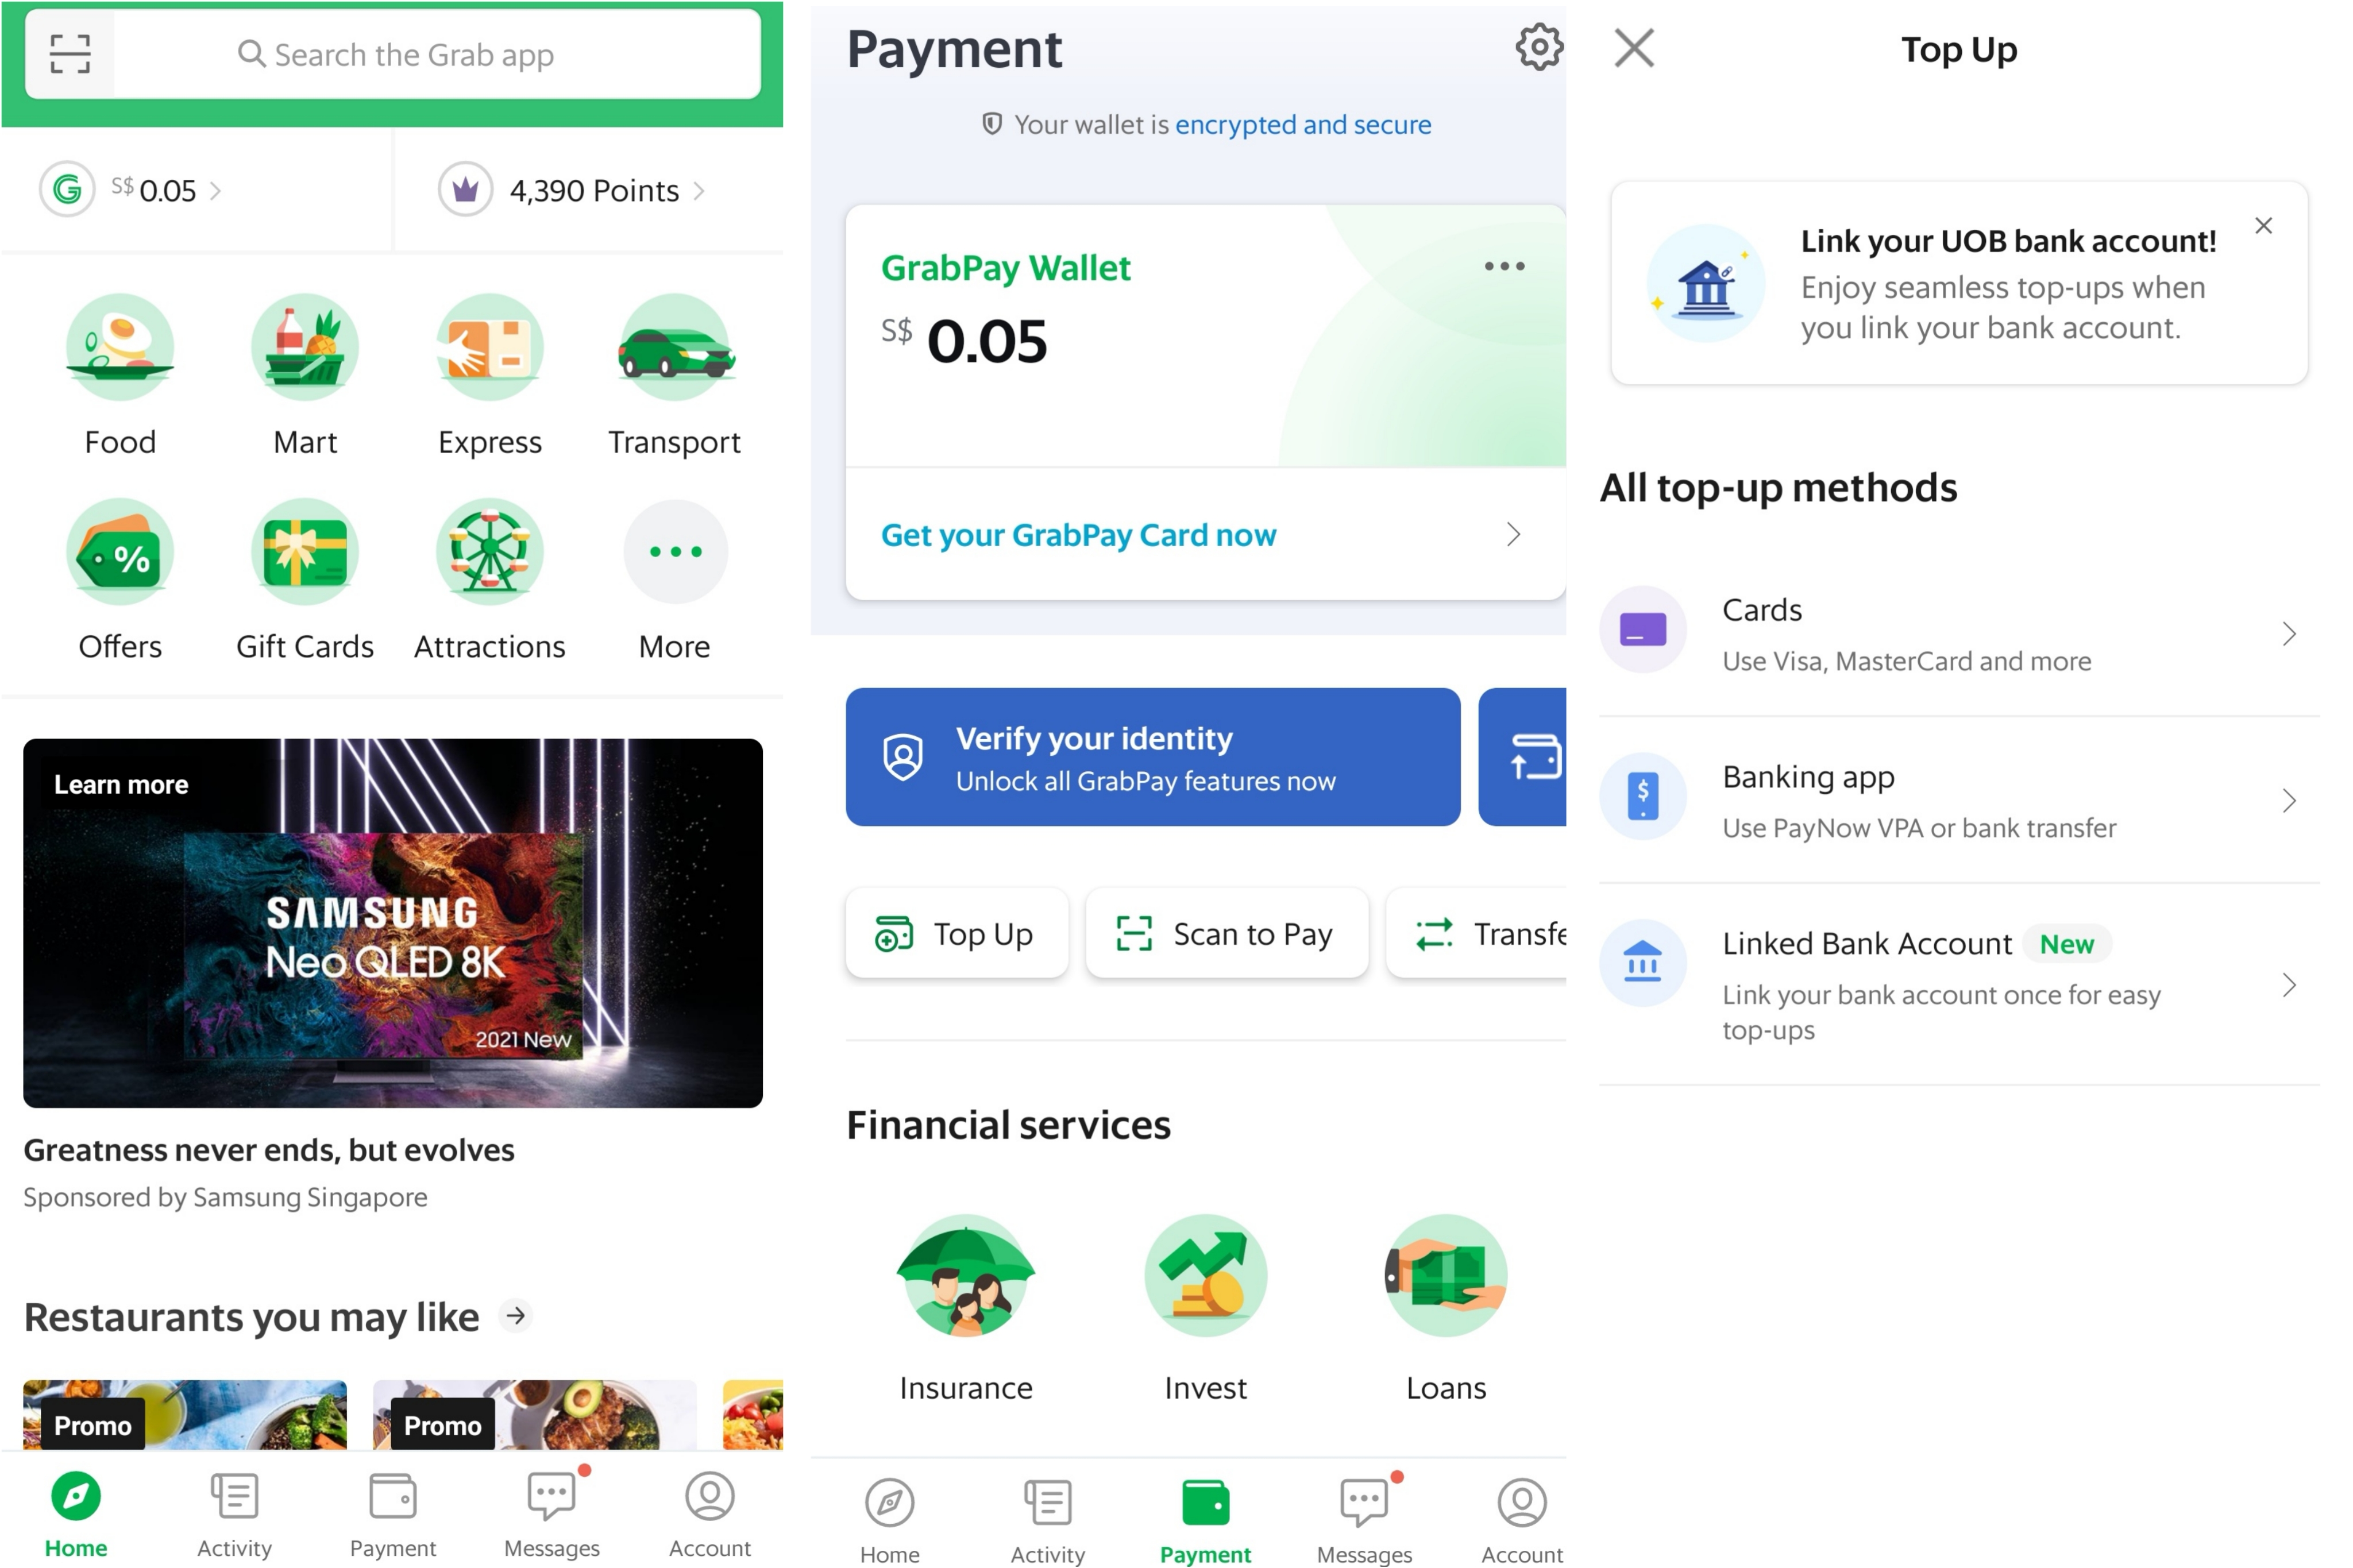
\includegraphics[height=6cm]{Figures/grab_wallet.jpg}
	\caption{The flow to find top-up option in Grab app}
	\label{fig:grab_wallet}
\end{figure}

\subsection{Improvements could be borrowed}
FSM app interface can be better designed to cope with the novices. There should be a direct interface of deposit account with transfer function in place. The transaction should be able to be done within the interface, with immediate feedback such as "Fund transfer successfully" and update the account balance. When the user has a goal (transfer fund to the platform), the interface should make it easy for user to "plan, specify and perform" the action with the interface, and also "perceive, interpret and compare" with the goal.[2] 

\section{References}
[1] Joyner, D. (2020). Designing with the Three Views. Udacity. 

https://classroom.udacity.com/courses/ud400/lessons/9044917867/concepts/

073deac0-9e73-4eae-9b3a-01ae17bf7e4e. 

[2] Joyner, D. (2020). Norman's Feedback Cycle Stages. Udacity. 

https://classroom.udacity.com/courses/ud400/lessons/9129419879/concepts/

063d8205-8902-47c1-939b-fc1151dacaa2. 

\end{document}